\documentclass[12pt, a4paper]{article}
% Verilog code formatting ref: https://tex.stackexchange.com/questions/377122/typesetting-for-a-verilog-lstinput
\usepackage{xcolor}
\usepackage{listings}
\definecolor{vgreen}{RGB}{104,180,104}
\definecolor{vblue}{RGB}{49,49,255}
\definecolor{vorange}{RGB}{255,143,102}

\lstdefinestyle{verilog-style}
{
    language=Verilog,    
    breaklines=true,    
    basicstyle=\small\ttfamily,
    keywordstyle=\color{vblue},
    identifierstyle=\color{black},
    commentstyle=\color{vgreen},
    numbers=left,
    numberstyle=\tiny\color{black},
    numbersep=10pt,
    tabsize=8,
    moredelim=*[s][\colorIndex]{[}{]},
    literate=*{:}{:}1
}

\definecolor{mGreen}{rgb}{0,0.6,0}
\definecolor{mGray}{rgb}{0.5,0.5,0.5}
\definecolor{mPurple}{rgb}{0.58,0,0.82}
\definecolor{backgroundColour}{rgb}{0.95,0.95,0.92}

\lstdefinestyle{CStyle}{
    backgroundcolor=\color{backgroundColour},   
    commentstyle=\color{mGreen},
    keywordstyle=\color{magenta},
    numberstyle=\tiny\color{mGray},
    stringstyle=\color{mPurple},
    basicstyle=\footnotesize,
    breakatwhitespace=false,         
    breaklines=true,                 
    captionpos=b,                    
    keepspaces=true,                 
    numbers=left,                    
    numbersep=5pt,                  
    showspaces=false,                
    showstringspaces=false,
    showtabs=false,                  
    tabsize=2,
    language=C
}

\makeatletter
\newcommand*\@lbracket{[}
\newcommand*\@rbracket{]}
\newcommand*\@colon{:}
\newcommand*\colorIndex{%
    \edef\@temp{\the\lst@token}%
    \ifx\@temp\@lbracket \color{black}%
    \else\ifx\@temp\@rbracket \color{black}%
    \else\ifx\@temp\@colon \color{black}%
    \else \color{vorange}%
    \fi\fi\fi
}
\makeatother
\usepackage{trace}

\setcounter{secnumdepth}{3} % To add subsubsections to the table of contents
% for QnA ref: https://latex.org/forum/viewtopic.php?t=10494
\newcounter{question}
\setcounter{question}{0}
\newcommand{\question}[1]{\item[\textbf{Q\refstepcounter{question}\thequestion.}] \textbf{#1}}
\newcommand{\answer}[1]{\item[Answer:] #1}


% A pretty common set of packages
\usepackage[margin=2.5cm]{geometry}
\usepackage[T1]{fontenc}
\usepackage[utf8]{inputenc}
\usepackage{blindtext}
\author{Maitreya Ranade}
\date{\today}
\usepackage{pdfpages}
\usepackage{graphicx}
\usepackage{amssymb}
\usepackage{amsmath}
\usepackage{color}
\usepackage{import}
\usepackage{booktabs}
\usepackage{multirow}
\usepackage{engord}
\usepackage{soul}
\usepackage{textcomp}
\usepackage{parskip}
\usepackage{setspace}
\usepackage{titlesec}
\usepackage{fancyhdr}
\usepackage{tabularx}
\usepackage{mathtools} % for '\DeclarePairedDelimiter' macro
\DeclarePairedDelimiter\norm\lVert\rVert
\usepackage{bookmark}
\pagestyle{fancy}
\usepackage[UKenglish]{babel}
\usepackage[UKenglish]{isodate}
\usepackage[skip=2pt,font=footnotesize,justification=centering]{caption}
\usepackage{natbib}
\usepackage{float}
\usepackage{dirtree}
\usepackage{url}
\usepackage{enumitem}
\usepackage{tgpagella}


% Custom environments
\newenvironment{highlight}
{\vspace{2mm} \hrule \vspace{2mm} \em}
{\vspace{2mm} \hrule \vspace{2mm}}


% Make some additional useful commands
\newcommand{\ie}{\emph{i.e.}\ }
\newcommand{\eg}{\emph{e.g.}\ }
\newcommand{\etal}{\emph{et al}}
\newcommand{\sub}[1]{$_{\textrm{#1}}$}
\newcommand{\super}[1]{$^{\textrm{#1}}$}
\newcommand{\degC}{$^{\circ}$C}
\newcommand{\wig}{$\sim$}
\newcommand{\ord}[1]{\engordnumber{#1}}
\newcommand{\num}[2]{$#1\,$#2}
\newcommand{\range}[3]{$#1$-$#2\,$#3}
\newcommand{\roughly}[2]{$\sim\!#1\,$#2}
\newcommand{\area}[3]{$#1 \! \times \! #2\,$#3}
\newcommand{\vol}[4]{$#1 \! \times \! #2 \! \times \! #3\,$#4}
\newcommand{\cube}[1]{$#1 \! \times \! #1 \! \times \! #1$}
\newcommand{\figref}[1]{Figure~\ref{#1}}
\newcommand{\eqnref}[1]{Equation~\ref{#1}}
\newcommand{\tableref}[1]{Table~\ref{#1}}
\newcommand{\secref}[1]{Section \ref{#1}}
\newcommand{\XC}{\emph{exchange-correlation}}
\newcommand{\abinit}{\emph{ab initio}}
\newcommand{\Abinit}{\emph{Ab initio}}
\newcommand{\Lonetwo}{L1$_{2}$}
\newcommand{\Dznt}{D0$_{19}$}
\newcommand{\Dtf}{D8$_{5}$}
\newcommand{\Btwo}{B$_{2}$}
\newcommand{\fcc}{\emph{fcc}}
\newcommand{\hcp}{\emph{hcp}}
\newcommand{\bcc}{\emph{bcc}}
\newcommand{\Ang}{{\AA}}
\newcommand{\inverseAng}{{\AA}$^{-1}$}
\newcommand{\comment}[1]{\textcolor{red}{[COMMENT: #1]}}
\newcommand{\more}{\textcolor{red}{[MORE]}}
\newcommand{\red}[1]{\textcolor{red}{#1}}
\newcommand{\SubItem}[1]{
    {\setlength\itemindent{15pt} \item[] \textbf{#1}}
}
% Change this to modify look of header and footer
\lhead{}
\chead{}
\rhead{}
\lfoot{}
\cfoot{\thepage{}}
\rfoot{}
\renewcommand{\headrulewidth}{0pt}
\renewcommand{\footrulewidth}{0pt}
\usepackage{hyperref}
\hypersetup{
    colorlinks=true,
    linkcolor=blue,
    filecolor=magenta,      
    urlcolor=cyan,
}
\urlstyle{same}
\newcommand{\foo}{\hspace{-2.3pt}$\bullet$ \hspace{5pt}}   % For timeline
  

\begin{document}
	\onehalfspacing
	Date: \today{} \hfill{} Name: Maitreya Ranade
	\begin{center}
		\topskip0pt
		\vspace*{\fill}
		{\LARGE C++ Language} \\
		% This report is written for personal understanding and not for publication or distribution.
		\vspace*{\fill}
	\end{center}
	
	\pagebreak
	\singlespacing
	\tableofcontents
	\pagebreak

    \section{C/C++ Preprocessors}

    As the name suggests Preprocessors are programs that process our source code before compilation. There are a number of steps involved between writing a program and executing a program in C / C++. 


    \begin{figure}[H]
        \begin{center}
            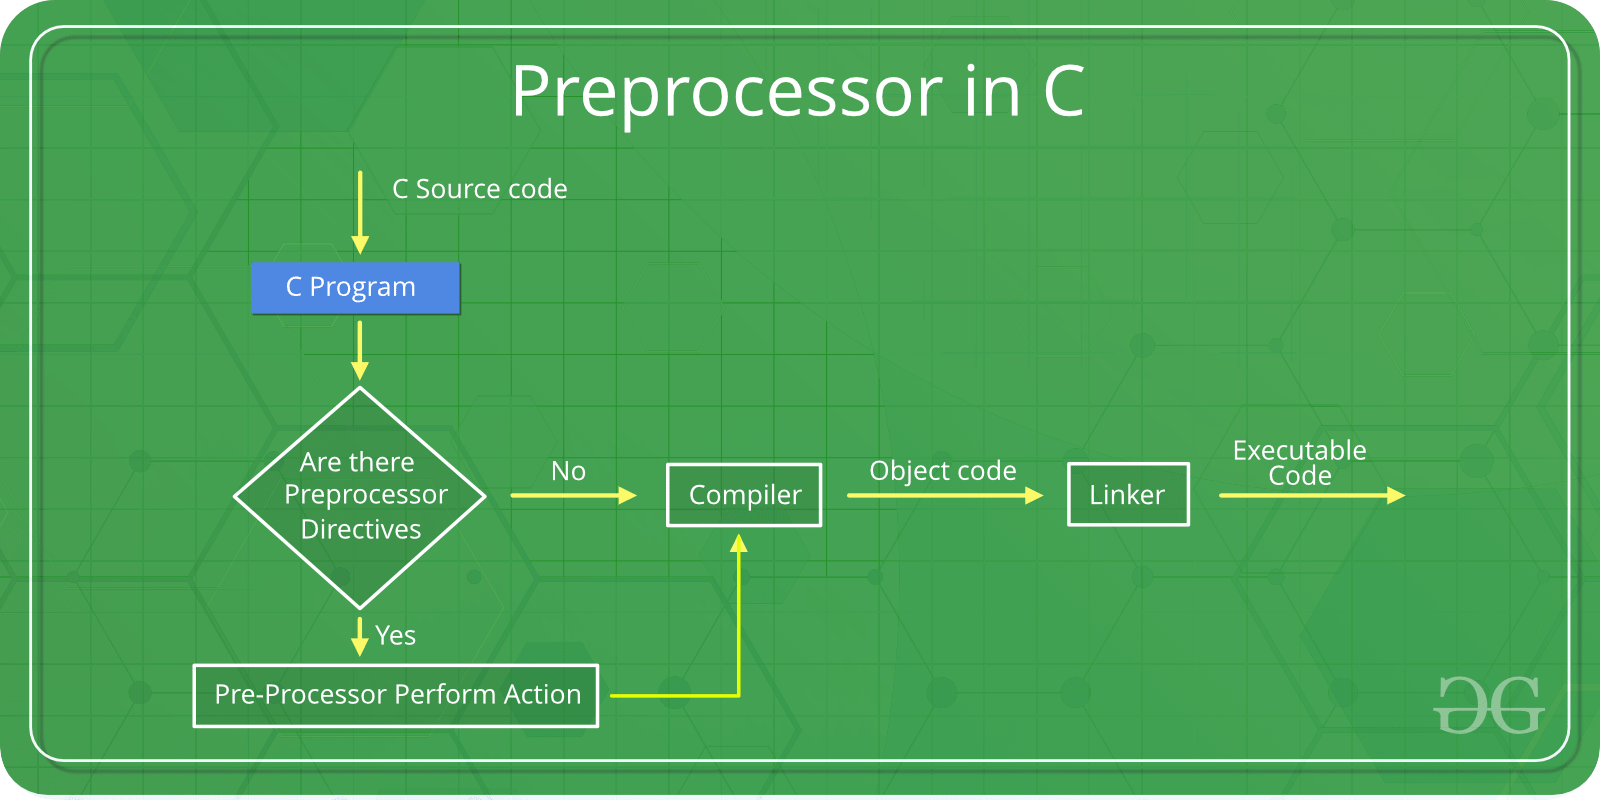
\includegraphics[width=0.6\textwidth]{images/Cpreprocessor.png}
            \caption{Preprocessor in C}
            \label{Cpreprocessor}
        \end{center}
    \end{figure}

    The source code file is processed by preprocessors and an expanded source code file is generated named program. This expanded file is compiled by the compiler and an object code file is generated named program .obj. Finally, the linker links this object code file to the object code of the library functions to generate the executable file program.exe.

    \par Preprocessor programs provide preprocessors directives which tell the compiler to preprocess the source code before compiling. All of these preprocessor directives begin with a '\#' (hash) symbol. The '\#' symbol indicates that, whatever statement starts with \#, is going to the preprocessor program, and preprocessor program will execute this statement. Examples of some preprocessor directives are: \#include, \#define, \#ifndef etc. Remember that \# symbol only provides a path that it will go to the preprocessor, and command such as include is processed by preprocessor program. For example, include will include extra code to your program. We can place these preprocessor directives anywhere in our program. 

    There are 4 main types of preprocessor directives: 
    \begin{enumerate}
        \item Macros
        \item File Inclusion
        \item Conditional Compilation
        \item Other directives
    \end{enumerate} 
    
    Macros: Macros are a piece of code in a program which is given some name. Whenever this name is encountered by the compiler the compiler replaces the name with the actual piece of code. The '\#define' directive is used to define a macro. 

    \begin{highlight}
        Note: There is no semi-colon(';') at the end of macro definition. Macro definitions do not need a semi-colon to end.
    \end{highlight}


    File Inclusion: This type of preprocessor directive tells the compiler to include a file in the source code program. There are two types of files which can be included by the user in the program: 
        Header File or Standard files: These files contains definition of pre-defined functions like printf(), scanf() etc. These files must be included for working with these functions. Different function are declared in different header files. For example standard I/O functions are in 'iostream' file whereas functions which perform string operations are in 'string' file.
        
        user defined files: When a program becomes very large, it is good practice to divide it into smaller files and include whenever needed. These types of files are user defined files. These files can be included as:


    Conditional Compilation: Conditional Compilation directives are type of directives which helps to compile a specific portion of the program or to skip compilation of some specific part of the program based on some conditions. This can be done with the help of two preprocessing commands 'ifdef' and 'endif'. 

    If the macro with name as 'macroname' is defined then the block of statements will execute normally but if it is not defined, the compiler will simply skip this block of statements. 

    Other directives: Apart from the above directives there are two more directives which are not commonly used. These are: 
    \#undef Directive: The \#undef directive is used to undefine an existing macro. This directive works as:

    Using this statement will undefine the existing macro LIMIT. After this statement every “\#ifdef LIMIT” statement will evaluate to false. 

    \#pragma Directive: This directive is a special purpose directive and is used to turn on or off some features. This type of directives are compiler-specific, i.e., they vary from compiler to compiler. Some of the \#pragma directives are discussed below: 
    \#pragma startup and \#pragma exit: These directives helps us to specify the functions that are needed to run before program startup( before the control passes to main()) and just before program exit (just before the control returns from main()). 
    Note: Below program will not work with GCC compilers. 
    Look at the below program:


    \#pragma warn Directive: This directive is used to hide the warning message which are displayed during compilation. 
    We can hide the warnings as shown below: 
    \#pragma warn -rvl: This directive hides those warning which are raised when a function which is supposed to return a value does not returns a value.
    \#pragma warn -par: This directive hides those warning which are raised when a function does not uses the parameters passed to it.
    \#pragma warn -rch: This directive hides those warning which are raised when a code is unreachable. For example: any code written after the return statement in a function is unreachable.


    \paragraph{Pragma Directive in C/C++}
    This directive is a special purpose directive and is used to turn on or off some features. This type of directives are compiler-specific i.e., they vary from compiler to compiler. Some of the pragma directives are discussed below:
    
    \#pragma startup and \#pragma exit: These directives helps us to specify the functions that are needed to run before program startup( before the control passes to main()) and just before program exit (just before the control returns from main()).
    Note: Below program will not work with GCC compilers.
    Look at the below program:
    
    \iffalse
        https://www.tutorialspoint.com/c-cplusplus-preprocessor-directives
        https://www.tutorialspoint.com/cplusplus/cpp_preprocessor.htm
        https://www.geeksforgeeks.org/cc-preprocessors/
        https://www.tutorialspoint.com/cprogramming/c_preprocessors.htm
    \fi


    \iffalse
    \section{Recursion}
    \section{Arrays}
    \section{Structure and union}
    \section{File handling}


    \chapter{Data Structures}    
    \section{Introduction}
    \section{Stacks}
    \section{Queues}
    \section{Linked Lists}
    \section{Trees}
    \section{Binary Search Trees}
    \section{Binary Heaps}
    \section{Graphs}

	\fi

    % \section{Programs in C}
    % \iffalse
pyramid of starts
palindrome check
armstrong number check
strong number check
prime number check
addition of 2 numbers
fibonacci series
Floyd's triangle
binary to decimal conversion
calculating power of an integer
check leap year
perfect number check
\fi

Star Pyramid Pattern 
\begin{lstlisting}[style=CStyle]
#include <stdio.h>  
#include <conio.h>  
void main()  
{  
    int i, j, rows;  
    printf (" Enter a number to define the rows: \n ");  
    scanf("%d", &rows);  
    printf("\n");  
    for (i = 1; i <= rows; ++i) // outer loop  
    {  
        for (j = 1; j <= i; ++j) // inner loop  
        {  
            printf ("* "); // print the Star  
        }  
        printf ("\n");   
    }  
    getch();      
}  
\end{lstlisting}
    % \clearpage

    \section{References}

	\begin{itemize} 
        \item \href{https://youtube.com/playlist?list=PLBlnK6fEyqRhX6r2uhhlubuF5QextdCSM}{Neso Academy (Youtube Channel) (C Programming \& Data Structures playlist)}
        \item Let us C by Yashwant Kanetkar    
        \item \href{https://www.tutorialspoint.com/cprogramming/index.htm}{Tutorials Point}
        \item \href{https://www.geeksforgeeks.org/c-programming-language/}{Geeks for geeks}
        \item \href{https://publications.gbdirect.co.uk/c_book/}{The C book}
	\end{itemize}
	
\end{document}




